\chapter{Experiments}
\section{Setup}
All the experiments were performed on a Lenovo G50-80 laptop with the following specifications:

\begin{itemize}
	\item Running Windows 10 x64
	\item CPU: Intel i5-5200U with 2 cores running at 2.20 GHz
	\item 4 GB RAM
\end{itemize}

The experiments were performed from IntelliJ with a maximum memory heap size of 2048 MB.
In all experiments, the algorithm was run five times on each input and we plotted the median runtime in the graph. By using the median value instead of the mean value, we avoid outliers affecting the graph. Such outliers could among other things be caused by the OS prioritizing other processes so ignoring these will give a more representative graph. Before each experiment, we ran the algorithm to be tested with random inputs \todo{20? or 100?} times in order to warm up the cache.

\section{The NLogN Algorithm}
We know that the runtime of the algorithm is $O(nlogn)$ for $n$ sized trees. However, we would like to find out how the algorithm runs in practice. How is the average runtime for random looking trees? What kind of trees give the best runtime? What kind of trees give the worst?

In the following sections we will walk through some of the experiments we did in order to answer these questions.

\subsection{Random Trees}
In practice, an algorithm like this will most likely be used on many very different looking trees. We therefore made an experiment to test how the runtime of the algorithm would look for randomly generated trees.

We ran the algorithm on randomly created trees of sizes $100, 200, ..., 80000$.

The result of this experiment is seen in Figure \ref{randomTreesGraph}. Since we expected the algorithm to have runtime $O(nlogn)$, we divided the runtime with $nlogn$ and the graph should be constant. However, this is not exactly what we see in the graph. There are three things to notice. First from size ~10000 to ~15000 the graph is growing, at size ~30000 and ~42000 the graph makes a sudden increase and afterwards decreases, and at ~80000 the graph again makes a sudden increase, but seems to keep increasing. A reason for this behaviour could be that the runtime is affected by the garbage collector working while the program is running. The garbage collector used in the execution is the default garbage collector for the JVM. This garbage collector pauses the program execution when collecting and therefore directly affects its runtime.

\begin{figure}
	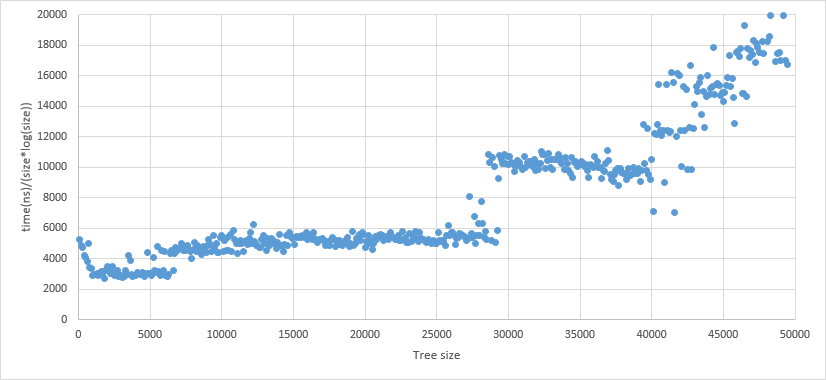
\includegraphics[width=\textwidth]{randomTreesGraph}
	\caption{The runtime of the $nlogn$ algorithm given random trees.}
	\label{randomTreesGraph}
\end{figure}

\subsubsection{Garbage Collecting}
We created a test to measure how much time was used by the garbage collector for each run of the algorithm. Again we created random trees of sizes $100, 200, ..., 80000$ and plotted the mean runtime of five runs for each tree size. Dividing the runtimes with $nlogn$ gave the graph shown in figure \ref{randomTreesGCGraph}. Here we see almost the exact same behaviour as for the runtime of the algorithm which indicates that the unexpected behaviour was all caused by the garbage collector. Figure \ref{randomTreesGCSubtractedGraph} shows a graph where the time used on garbage collecting is subtracted from the time used on running the algorithm. This graph looks more like what we expected of the algorithm and suggests that the runtime of the algorithm is indeed $O(nlogn)$.

\begin{figure}
	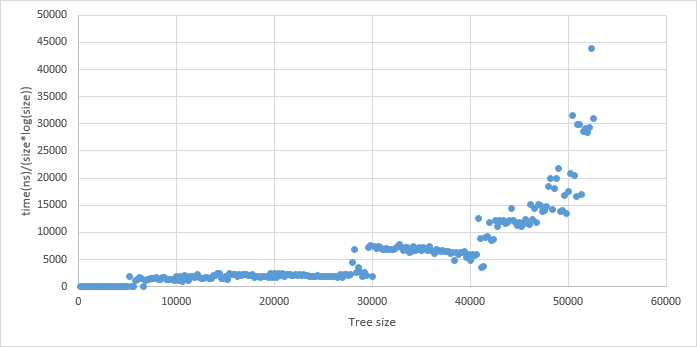
\includegraphics[width=\textwidth]{randomTreesGCGraph}
	\caption{The runtime of the garbage collector when running the $nlogn$ algorithm given random trees.}
	\label{randomTreesGCGraph}
\end{figure}

\begin{figure}
	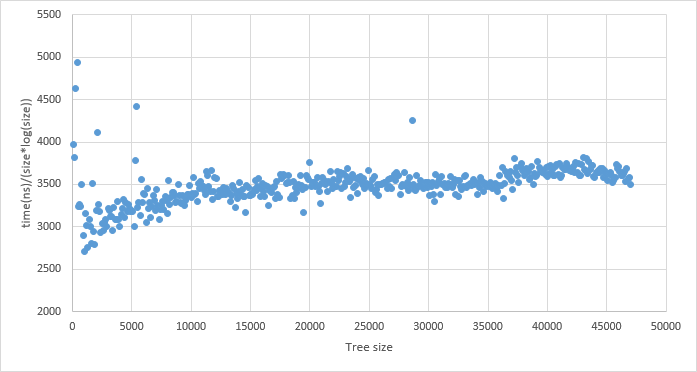
\includegraphics[width=\textwidth]{randomTreesGCSubtractedGraph}
	\caption{The runtime of the $nlogn$ algorithm given random trees after subtracting the time used on garbage collecting.}
	\label{randomTreesGCSubtractedGraph}
\end{figure}

Yet we still want to be able to explain this behaviour of the garbage collector, e.g. why the amount of work needed by the garbage collector increases at those exact tree sizes. So we tried running the same test again, but with a different amount of allocated memory. In the previous tests, a memory heap of 2048 MB were allocated. In \todo{figure ??} we see the result of the same test, but with a memory heap of 1024 MB allocated. In this experiment, we see the same increases in runtime of the garbage collector, but they happen earlier than in the previous experiment. This indicates that the garbage collector used in these experiments will run depending on how much free memory is left. Using a computer with more RAM so that a larger memory heap can be used could therefore result in a better runtime for large input trees. The algorithm should also be able to work for input trees larger than 80000 when allocating more than 2048 MB of memory.

\subsection{Best Case Trees}
The part of the algorithm that requires most processing power is creating the matching graphs and processing them to compute largest weight agreement matchings. Matching graphs consists of edges and computing LWAMs is done by processing these edges. A tree structure that minimizes the runtime of the algorithm is therefore a tree structure that minimizes the number of edges that needs to be created.

Recall how the edges are determined. For each leaf in $T_2$, an edge will be created for each centroid path encountered from the leaf to the root of $T_2$. For any two trees $T_1$ and $T_2$ that are given the algorithm, at least one edge will be created for each leaf of $T_2$ since all leaves will encounter the centroid path starting at the root of $T_2$. The number of edges created will therefore be minimal when $T_2$ has as few centroid paths as possible. Having a tree structure where each internal node has a leaf as one of its children, $T_2$ will have only one centroid path, so only one edge will be added for each leaf in $T_2$.

The process of creating edges is however done in every recursive call of the algorithm, so we want a structure of $T_1$ that gives the fewest possible recursive calls. Choosing the same tree structure as for $T_2$ means that each side tree of $\pi$ will have size 1 so there will be no recursive calls. We therefore expect this tree structure to give the shortest runtime of the algorithm.

When processing a matching graph $G(x)$ to compute LWAMs, each edge $(u_i, v_j)$ is processed where the leaf in the search tree corresponding to $v_j$ is searched for which takes $O(log\frac{|T_2(x)|}{n_j})$ time. Having input trees of the structure just mentioned, means that there is only one graph $G(r)$, where $r$ is the root of $T_2$, and for each node $v_j$, $n_j = 1$. So even with this tree structure, the total runtime of the algorithm is $\sum_{v_j \in \pi(r)} O(log n) = O(nlogn)$. We therefore don't expect an asymptotic improvement of the runtime compared to the result with random trees, but we do expect a noticeable constant improvement.

Another thing about the input trees that affects the runtime of the algorithm, is how similar the two trees are. The more they have in common, the larger the LWAMs will become, and processing these LWAMs will take more time. Even though the algorithm will probably be used for trees that look alike in practice, it will be fastest for trees that doesn't. Again we don't expect an asymptotic improvement compared to using identical trees, but a slight constant improvement.

We created an experiment for running the algorithm on trees of the structure explained earlier where the two trees were identical, and one where the leaves in the second tree appeared in the opposite order than that of the first tree.

The graph(s) in \todo{Figure ??} shows the runtime of the algorithm, using the two kinds of inputs just explained. As expected, it looks very much like the algorithm is running in $O(nlogn)$ time, but it is still significantly faster than what we saw for random tree inputs. \todo{compare the two graphs}

Another thing to notice is that we don't see the sudden increases in runtime as we did when inputting random trees. This can be due to the fact that there are no recursive calls meaning that the program does not use up memory on side trees, induced subtrees etc. Therefore the garbage collector has less work to do.

\todo{investigate overall space consumption}

\subsection{Worst Case Trees}
Since the runtime of the algorithm can be minimized by inputting trees that minimizes the number of edges created, we expect that the input trees that gives the worst runtime are trees that maximizes the number of edges that is created by the algorithm.

Again, recall that for each leaf in $T_2$, an edge will be created for each centroid path encountered from the leaf to the root of $T_2$. Now consider the centroid path $\pi(r)$ with nodes $v_1, v_2, ..., v_q$ starting at the root node $r$, where $q \ge 4$. The leaf $v_q$ will encounter only one centroid path on the path to $r$, namely $\pi(r)$ no matter the structure of $T_2$, so a single edge is created. The side tree $N_{q-1}$ is a single leaf. Otherwise $\pi(r)$ would include the root of $N_{q-1}$ instead of $v_q$. That leaf also encounters exactly one graph. The side tree $N_{q-2}$ contains at most 2 leaves or $\pi(r)$ would have included the root of $N_{q-2}$ instead of $v_{q-1}$. If $N_{q-2}$ is a single leaf, it will encounter only one centroid path, but if $N_{q-2}$ contains 2 leaves, both leaves will encounter 2 centroid paths. Continuing this way we show that in order to maximize the number of edges created in the algorithm, each side tree of the centroid paths of $T_2$ should hold as many leaves as possible. Creating $T_2$ with this in mind, results in a complete binary tree.

Now let's consider the structure of $T_1$. Since the process of creating edges is done in every recursive call of the algorithm, we want a structure of $T_1$ that results in as many recursive calls as possible with the largest possible trees. A recursive call is made for each side tree of $\pi$, so making these as large as possible will result in the most edges being created. This means that also $T_1$ should be a complete binary tree.

To verify the runtime of these kind of input trees, we created an experiment for running the algorithm with only complete binary trees as input. \todo{identical trees or spread out leaf names in T1?}

The graph in figure \ref{completeIdenticalTreesGraph} shows the result of this experiment. It is easily seen that the runtime is worse than when inputting random trees, and again we see sudden increases in runtime when reaching certain tree sizes. Already at tree size ~22000, the JVM ran out of memory and could not continue the execution. Since this tree structure is maximizing the amount of recursive calls and the size of the trees it also means that the amount of memory needed by the algorithm is maximized. Therefore the garbage collector will need to run more often and could cause the unexpected increase in runtime. The graph in figure \ref{completeIdenticalTreesGCGraph} shows the runtime of the garbage collector during the experiment and \todo{Figure ??} shows the runtime of the algorithm after having subtracted the runtime of the garbage collector. \todo{explain}

\begin{figure}
	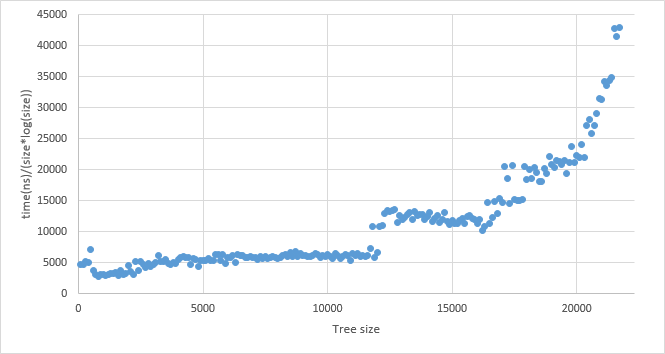
\includegraphics[width=\textwidth]{completeIdenticalTreesGraph}
	\caption{The runtime of the $nlogn$ algorithm given two identical complete trees.}
	\label{completeIdenticalTreesGraph}
\end{figure}

\begin{figure}
	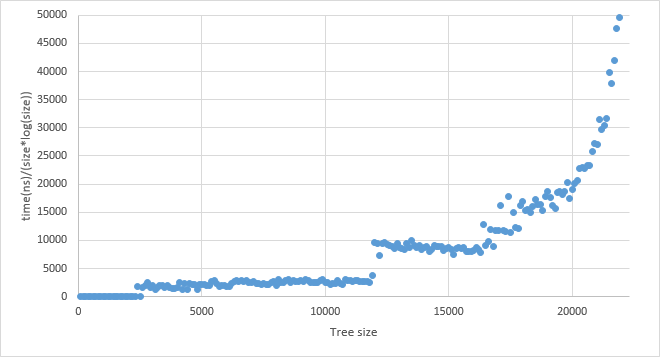
\includegraphics[width=\textwidth]{completeIdenticalTreesGCGraph}
	\caption{The runtime of the garbage collector when running the $nlogn$ algorithm given two identical complete trees.}
	\label{completeIdenticalTreesGCGraph}
\end{figure}

\todo{Graph with all experiment results}

\subsection{Induced Subtrees}
A requirement for the algorithm was that any tree $T$ can be preprocessed in $O(|T|)$ time, such that for any subset $L$ of its leaves, the subtree induced by $L$ can be computed in $O(|L|)$ time.

In order to verify that this was satisfied, we created a test for the runtime of the preprocessing and two tests for the runtime of the computation of the induced subtrees.

\subsubsection{Preprocessing}
Since the preprocessing is done by simply traversing the input tree and preprocessing the tree for LCA queries (which we know is done in $O(|T|)$ time), the structure of the tree does not affect the runtime. We therefore tested the runtime for random trees of sizes between 1000 and 100000. Dividing the runtime with the size of the input tree gave the graph in \todo{figure ??} which indeed looks constant.

\subsubsection{Inducing}
To verify that the runtime is not affected by the size of the tree, we tested the runtime for random trees of sizes between 1000 and 100000 and a constant number of input leaves. The test result is plotted in the graph in \todo{figure ??}.

To verify that the runtime is linear w.r.t. the number of input leaves, we tested the runtime for a tree of size 100000 and input leaves of sizes between 100 and 100000. Dividing the runtime with the number of input leaves gave the graph in \todo{figure ??}.



